\section{Metod}
\label{sec:joel_o-method}
För att svara på frågeställningarna har information från flera källor inhämtats. En udersökning av olika Javascript-projekt har gett kvantitativa data om dess beroenden. Denna har kompletterats information från tidigare forskning och erfarenheter från det utförda projektet för att ge en helhetsbild över beroendens påverkan.

\subsection{Analys av Javascript-projekt}
I denna anlys har beroenden för 1000 open-source projekt från GitHub undersökts. Ett script skrivet i Python 3 har använts för att hämta och hantera data. För lagring av data lokalt har en SQLite-databas använts. Detta är en lättviktig realtionsdatabas som enkelt kan ändras från Python-scriptet. Scriptet som har använts, loggar från körningar och den slutgiltiga databasen finns på GitHub\footnote{https://github.com/joelnir/dependency-analysis}..

I databasen skapades tabeller för att spara data om Javascript-projekt, npm-paket och relationer mellan dem. Tabeller för intressant statistik så som hur många versionsreferenser som var ogiltiga skapades också. Ett diagram över databasen visas i figur \ref{fig:dependency-db}.

\begin{figure}[h]
  \centering
  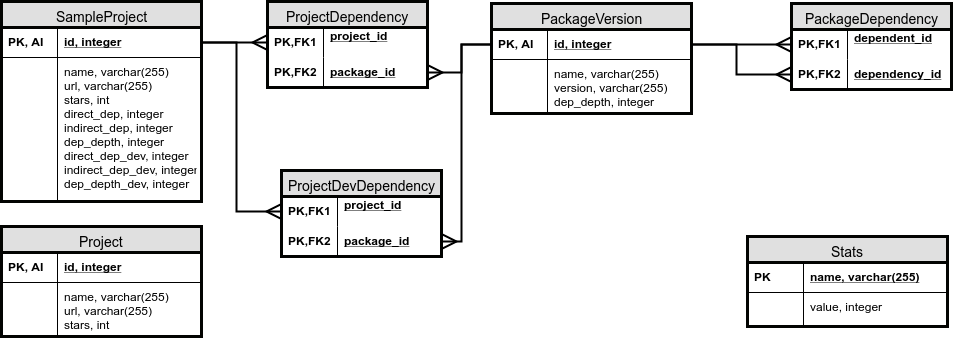
\includegraphics[scale=0.42]{npm_db}
  \caption{Databasen som har använts under undersökningen}
  \label{fig:dependency-db}
\end{figure}

Tabellerna innehåller följande:

\begin{enumerate}[leftmargin=3cm]
  \item [\textbf{Project}] Samtliga projekt som övervägs för undersökningen
  \item [\textbf{SampleProject}] Det urval av 1000 projekt som undersöks
\end{enumerate}

Då analysen enligt frågeställning \ref{joel_o-fs:1} ska utföras på populära Javascript-projekt behöver populäritet först definieras. GitHubs system med stjärnor valdes som ett bra mått på populäritet. Projekt med mer än 500 stjärnmarkeringar definierades som populära. Denna gräns är godtycklig, men den ger en stor datamängd att utgå ifrån.



\subsection{Informationsinsamling}

\subsection{Projekterfarenheter}

Tanken är att samla in data genom att skriva ett script som går igenom repositiories för open-source javascript projekt. En begränsad mängd av projekt att undersöka kan väljas genom att exempelvis se till de högst rankade projekten på github. Hur detta urval görs är dock viktigt och bör poängteras noga.

Själva datainsamlingen kan göras genom att i dessa  projekt läsa av deras beroenden från filen package.json, som används av npm. Detta ger direkta beroenden.

Hela trädet av beroenden kan fås från package-lock.json, som ofta lagras tillsammans med package.json. Detta ger indirekta beroenden och det kan vara möjligt att göra vidare undersökningar på denna graf (exempelvis nivåer av beroenden)

För att få fram inforamtion om effekterna av beroenden får en större informationssökning genomföras. Det verkar finnas gott om akademiska källor av intresse för detta och troligen även bloggposter från personer med stor erfarenhet av javascript-projekt (som kan användas ur ett kritiskt perspektiv).

Till viss del kan den egna gruppens erfarenheter presenteras. Det vore även möjligt att intervjua någon/några från en annan grupp inom kursen och därmed få in en större bredd av erfarenheter.\\

\textbf{Här följer några källor som kan användas}\\
\href{https://dspace.cvut.cz/bitstream/handle/10467/68195/F8-DP-2017-Zitny-Jakub-thesis.pdf?sequence=1&isAllowed=y}{Liknande undersökning}\\
\href{https://arxiv.org/pdf/1709.04638.pdf}{Effekter av micro-paket i npm}\\
\href{https://repository.tudelft.nl/islandora/object/uuid:3a15293b-16f6-4e9d-b6a2-f02cd52f1a9e?collection=education}{Effekter av beroenden i npm för säkerhet}\\ \href{https://arxiv.org/pdf/1710.04936.pdf}{Jämförelse mellan pakethantering i olika programmeringsspråk}\\ \href{http://www.scotthenry.ca/wp-content/uploads/2018/01/Report.pdf}{Undersökning om uppdatering av beroenden i npm}\\
